\documentclass{article}
\title{Twiddle -- A DSL for the Functional Bit-hacker}
\author{Michael Buch}

\usepackage[inline]{enumitem} % inline numbered lists
\usepackage[left=2cm,right=2cm]{geometry}
\usepackage{verbatim} % for comments
\usepackage{graphicx}
\usepackage{listings}
\usepackage{color}

\definecolor{dkgreen}{rgb}{0,0.6,0}
\definecolor{gray}{rgb}{0.5,0.5,0.5}
\definecolor{mauve}{rgb}{0.58,0,0.82}
\lstset{frame=tb,
  language=Scala,
  aboveskip=3mm,
  belowskip=3mm,
  showstringspaces=false,
  columns=flexible,
  basicstyle={\small\ttfamily},
  numbers=none,
  numberstyle=\tiny\color{gray},
  keywordstyle=\color{blue},
  commentstyle=\color{dkgreen},
  stringstyle=\color{mauve},
  breaklines=true,
  breakatwhitespace=true,
  tabsize=3
}

\begin{document}
\maketitle
\frenchspacing

\begin{abstract}
It is useful (and fun!) to bit twiddle i.e. perform arithmetic and manipulate data at the granularity of individual bits. Traditionally there is a compromise one has to make between using a low-level unsafe language that allows bit-twiddling versus a safe high-level language in which the type system or language design prohibit operations at bit-level (without additional complexity). The \textit{Twiddle} domain-specific language (DSL) is an embedded language written in Scala that generates bit-twiddling style C code. The language offers several modes of operation, useful for quick prototyping, debugging and custom extensions:
\begin{enumerate*}[label=(\arabic*)]
	\item Tracing interpreter
	\item Scala evaluator
	\item Twiddle AST generator
	\item C code generator
\end{enumerate*}.
Thus our language is a tool for the curious, a tool for safe bit-hackers and a tool for someone looking to get a bit more performance out of his high-level language.
\end{abstract}

\section{Motivation}
No need to worry about syntax such as semicolons, operator precedence, asterisk locations or qualifier usages.
\section{The Language \& Architecture}
\begin{figure}[t]
	\centering
	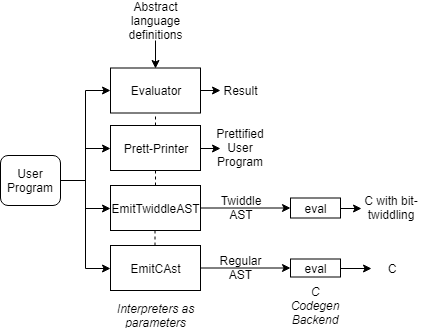
\includegraphics[scale=1]{twiddle_arch.png}
	\caption{Architecture of the Twiddle framework}\label{twiddle_arch}
\end{figure}
\subsection{Core}
The core of the language is split into modular pieces of functionality implemented as traits. As is common practice with tagless final interpreters (see section \ref{subsec:tagless}) we parameterize each set of language features with an evaluator that describes how each feature within its context. The core set of features is divided into following traits:
\begin{enumerate}
	\item Arithmatic
	\item Strings
	\item Bools
	\item Lambda
	\item LispLike
	\item CLike
	\item CMathOps
	\item CStrOps
\end{enumerate}

\subsection{Evaluators}
Each term in the language is a function whose parameters and return type are wrapped in the abstract type of the interpreter that is evaluating the function. The second column of figure \ref{twiddle_arch} shows the current set of supported interpreters.

\textit{Evaluator} corresponds to the \texttt{implicit object Eval} in \textbf{interpreter.scala}. Here terms are evaluated and returned as values in the host language (i.e. Scala).

\textit{Pretty-Printer} corresponds to the \texttt{implicit object Show} in \textbf{interpreter.scala}. Here all terms are of type \texttt{String} and evaluation of a term yields its pretty-printed version.

\textit{EmitTwiddleAST} corresponds to the Scala object of the same name in \textbf{codegen.scala}. This is the core of the Twiddle code generator.

\section{Codegen}
\subsection{Twiddle AST}
The code generation part of the Twiddle framework is shown in the bottom two branches of the flow chart in figure \ref{twiddle_arch}. As a way to map modularly and extensibly between a high-level language like the lambda calculus variant in our case to a low-level language like C we introduced a intermediate representation (IR) of the user-level Twiddle code structured as an abstract syntax tree (AST). The IR language includes features that would not fit to the semantics of the high-level language but are needed for bit-twiddling or general operations in C. Nodes in the AST are all represented by the \texttt{abstract trait Term} and evaluation of the terms occurs on nested tuples of terms (i.e. \texttt{Tup(Term, Tup(Tup(Term, Term)...)...)}) to be able to conveniently manipulate it from within the evaluator of the AST. Where there is only a small set of one-to-one mappings between terms in the object language and actual C language constructs, the IR mimics a subset of valid terms in C. Figure DIAGRAM NEEDED shows valid terms in the Twiddle IR. Distinction between primitives, expressions, C language identifiers, etc. is not provided since our evaluators on the AST did not require it. The term types can, however, be refined with additional traits if one needs to special-case according to certain classes of C language features.

As implied above, not all IR terms are features in the core language, thus terms such as \texttt{Ref(e: Term)} or \texttt{Assign(v: Term, e: Term)} are helper terms used to ease the transition from user-level language to C.

Arithmetic/Math operations
Variable declarations and assignment
Twiddle built in functions
\subsection{Twiddle AST Interpreters}
Gensym
Return helper
Lambda/apply
IO
Ensuring correct syntax
\section{Design Choices}
\subsection{Language Embedding}
\subsection{Scala}
\subsection{Tagless Final Style}\label{subsec:tagless}
\section{Conclusion \& Future Work}
\begin{itemize}
	\item Benefits of shallow embeddings. Can fall back to scala features. Don't need to implement side effects in object language necessarily.
	\item Extend LMS
	\item Use tagless evaluator for AST evaluation
	\item Writing larger programs
	\item Other backends
\end{itemize}

\bibliographystyle{ieeetran}
\bibliography{twiddle}
\end{document}